\documentclass[../thesis]{subfiles}

\begin{document}
	\chapter{Future Work}
	\label{chp:futurework}

	As is typical in research projects, several paths, either available from the start or unveiled with the progress, were not taken during this dissertation due its natural time constraints. Those paths, left for future work, are described in this chapter.

	First of all, all the implementations presented in this document could be integrated in a single software package (such as \blas library) supporting the three studied environments. In order for such a package to be useful though, the restrictions imposed by the assumptions presented in \label{sec:multicore:column} would have to be lifted by extending the implementations for complex arithmetic and to allow for quasi-triangular matrices,and by adding the Schur decomposition to allow for any matrix.

	Given the success of the results obtained with the multicore implementation and, in contrast, the lack of performance found in the implementations for the two hardware accelerators, an \mpi implementation of the algorithm might prove itself more efficient. Distributing the matrix through the available nodes, having each compute part of a diagonal using the multicore implementation and communicate only that part to the remaining nodes, and reducing the number of nodes involved gradually (as the size of the diagonal decreases) has the potential to replicate the results obtained with the benefits of increasing the parallelism through a \hetplat.

	Alternatively, using only one computational node for iterating over the diagonals but having the remaining nodes cooperating in the computation of the dependencies could also prove to be efficient, but it would more complex. An hybrid solution would also be interesting, by having less nodes computing the diagonal as the algorithm progresses but having the increasing idle nodes cooperating to solve the dependencies.

	As for the implementation using \intel\mic devices, further profiling, now using the command-line tool for \intel\vtune Amplifier, would reveal why the achieved performance was not able to surpass the multicore implementation. In particular, it would be interesting to use hardware events to examine how memory is used by the algorithm. If confirmed to be the bottleneck, a diagonalized rearrangement of the matrix could make the algorithm more efficient, at the expense of a preparation and cleanup step that, unlike what happens with ``blockification'', would almost certainly not be useful for any other linear algebra routines.

	Although OpenMP (specification 3.1) does not include any way to control thread affinity, \intel's OpenMP library was found to contain a mechanism for it through an environment variable (\texttt{KMP\_AFFINITY}) \cite{PRACE:MIC:BestPracticeGuide}. Nonetheless this mechanism was found to be confusing, and, consequently, the learning curve was assumed to be too steep for the project time-frame. A recent technical report \cite{CESGA:MIC:Evaluation} provides visual explanations for this mechanism contradicting that assumption. It is expectable that a balanced affinity policy, where the threads are spread amongst the cores but grouped sequentially by ID when the number of demanded threads exceeds the number of cores, with any granularity would achieve higher efficiency due a better usage of the first levels of cache.

	\begin{figure}
		\begin{center}
			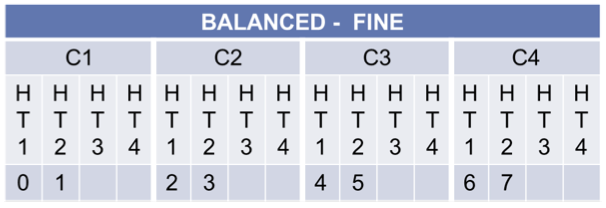
\includegraphics[width=\textwidth]{assets/images/kmp_affinity_balanced.png}
		\end{center}
		\caption{Example of balanced policy in a 4 core coprocessor for 8 threads with granularity fine (source: \cite{CESGA:MIC:Evaluation})}
		\label{fig:kmp_affinity:balanced}
	\end{figure}

	Nested parallelism in an OpenMP application is supposed to be something trivial, requiring only to create a parallel zone inside another. Yet, it was found to be disabled by default, focusing the entire parallelism in the outer parallel region \cite{PRACE:MIC:BestPracticeGuide}. In order to enable nested parallelism with OpenMP, it has to be explicitly enabled through the environment (or, alternatively, with a minimal change to the source code) and requires the number of threads to be set for each level (comma separated values through the environment or by using the appropriate function in the source code). Although this correction is quite easy, the problem was found after the optimizations described in \cref{sec:mic:optims} were implemented and tested. The time it required to rerun the performance tests would have to be taken from the \cuda implementation, which would probably never reach a functional state in such case. Consequently, it is left for future work.

	\tdr{Remove the OpenMP whining above}
	Regarding both \cref{chp:multicore,chp:mic}, correcting the mistake made with nested parallelism and performing experiments with thread affinity properly defined would be interesting enough to make it a priority. The balanced thread affinity policy with \intel's OpenMP library is expected to be the decisive step to take the implementation to equivalent levels in both \xeon processors and \intel\xeonphi coprocessors. Correcting the usage of nested parallelism should then give the implementation the final boost to finally take advantage of the resources made available in the coprocessor.

	Given that there was only opportunity to explore the native execution mode of the \intel\xeonphi coprocessor, it would be interesting to explore offload in the future. Similarly, if an \mpi implementation proves to be efficient the question remains whether using the coprocessor, either as another node or as an offload device, improves efficiency. The usage models for \intel\mkl are also intriguing unexplored paths. The compiler assisted offload, in particular, due to the advantage of allowing for data persistence, is expected to improve performance because the device would be focused entirely on executing routines already optimized for it. At the same time, the multiple parallel calls to these routines from the host when computing an entire diagonal of blocks in parallel could cause most of the work to be performed in host due to the unavailability of resources in the device, thus reducing the advantage of using the coprocessor.

	Specifically for the \cuda implementation, the optimizations described in \cref{sec:cuda:further} are left for future work due. Additionally, an optimized \blas package for single-block to replace the routines implemented in \cref{sec:cuda:blas} would improve the efficiency of the implementations using \gpus. Although these routines were implemented with performance in mind, there was no opportunity for deep profiling and improvements.

	Lastly, for both devices studied during this dissertation, implementations executing in the \cpus and the accelerator at the same time would hardly achieve higher speedups because of the synchronization required between the diagonals. Nevertheless, an hybrid implementation starting in the device and moving to the \cpu when the algorithm lacks the required parallelism could merge the best performance of both worlds. Alternatively, if such model proved to be efficient using the \intel\xeonphi coprocessor, \nvidia\gpus could be used only to offload \blas and \lapack routines, allowing for already existing optimized packages to be used \cite{NVIDIA:CUBLAS:5:0,PLASMA:MAGMA,CULA:LAPACK}.
\end{document}
